\documentclass{standalone}

%----------------------------------------------------------------------------------------------%
%                                 Packages and basic declarations
%----------------------------------------------------------------------------------------------%

\usepackage{amsmath}
\usepackage{mathrsfs}
\usepackage{pgf}
\usepackage{tikz}
\usepackage{verbatim}


\usetikzlibrary{arrows}



%----------------------------------------------------------------------------------------------%
%----------------------------------------------------------------------------------------------%
%                                            DOCUMENT STARTS
%----------------------------------------------------------------------------------------------%
%----------------------------------------------------------------------------------------------%


\begin{document}
 
\begin{tikzpicture}[scale=3]

%Tikz axis starts%

%\draw[->,black, line width = 5pt] (-4,0) -- (-4,3);
%\draw[->,black, line width = 5pt] (-4,0) -- (-4,-3);
%\node  at (-4,0) {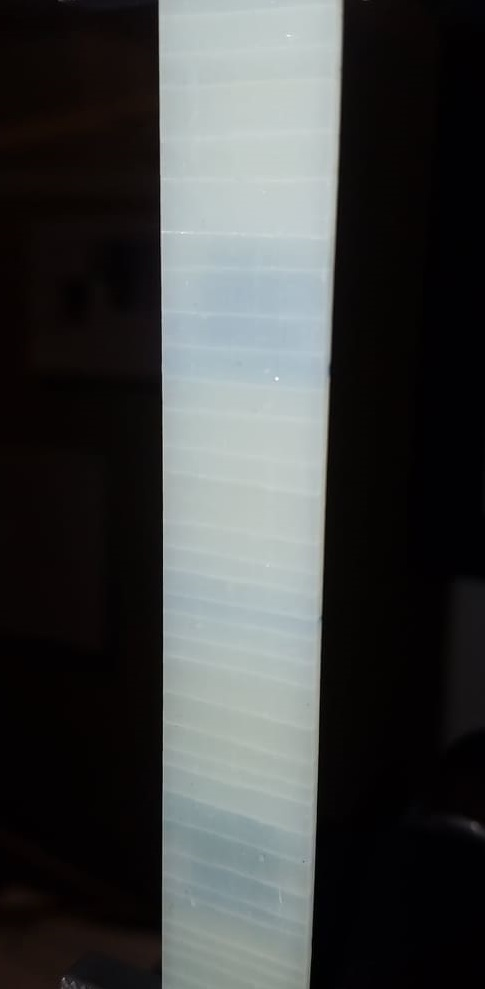
\includegraphics[height=0.6\textheight]{0-90_2_symm}};
%\draw[<->,red, line width = 1.25pt] (-4.35,-0.5) -- (-3.65,-0.625);
%\node[red, below]  at (-4,-0.65) {\tiny$\mathbf{\sim 15\ mm}$};
%\node[above, right]  at (-3.8,3) {\Huge$\mathbf{\varepsilon}$};
%\node[below, left]  at (-4.2,-3) {\Huge$\mathbf{\varepsilon}$};

\draw[->,black, line width = 5pt] (-2,0) -- (-2,3);
\draw[->,black, line width = 5pt] (-2,0) -- (-2,-3);
\node  at (-2,0) {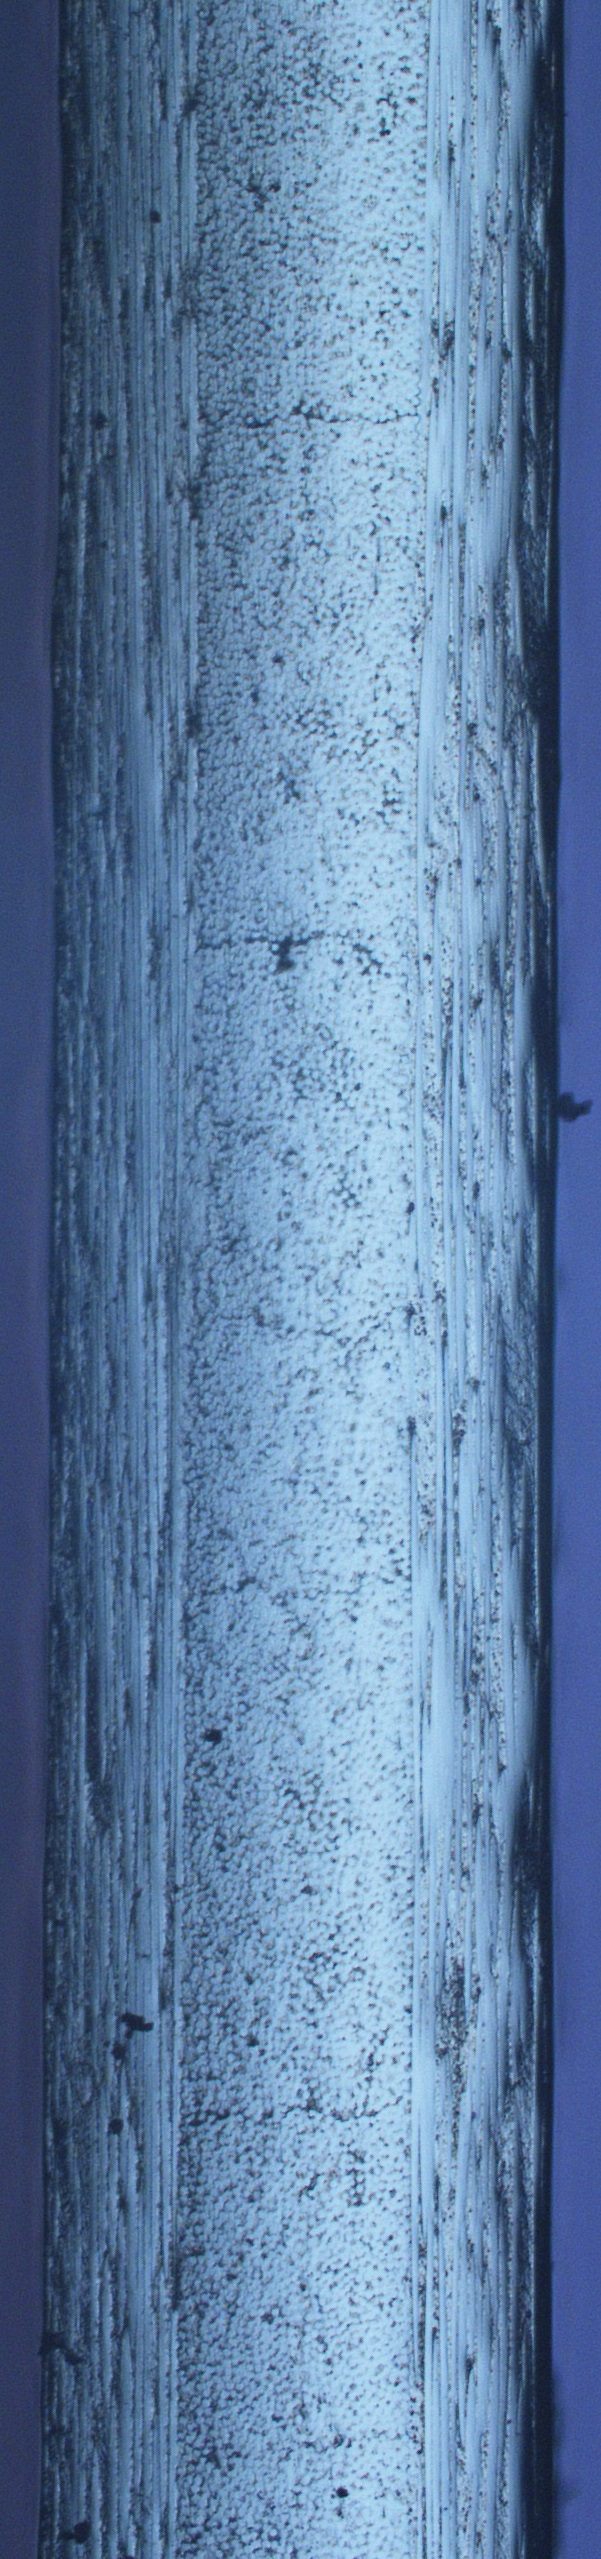
\includegraphics[height=13.75cm]{0-90_symm_edge}};
\draw[<->,red, line width = 1.25pt] (-2.46,-0.6) -- (-1.55,-0.6);
\node[red, below]  at (-2,-0.625) {\Huge$\mathbf{\sim 2\ mm}$};
\node[above, right]  at (-1.8,3) {\Huge$\mathbf{\varepsilon}$};
\node[below, left]  at (-2.2,-3) {\Huge$\mathbf{\varepsilon}$};

%\draw[->,black, line width = 5pt] (1,0) -- (1,3);
%\draw[->,black, line width = 5pt] (1,0) -- (1,-3);
%\node  at (1,0) {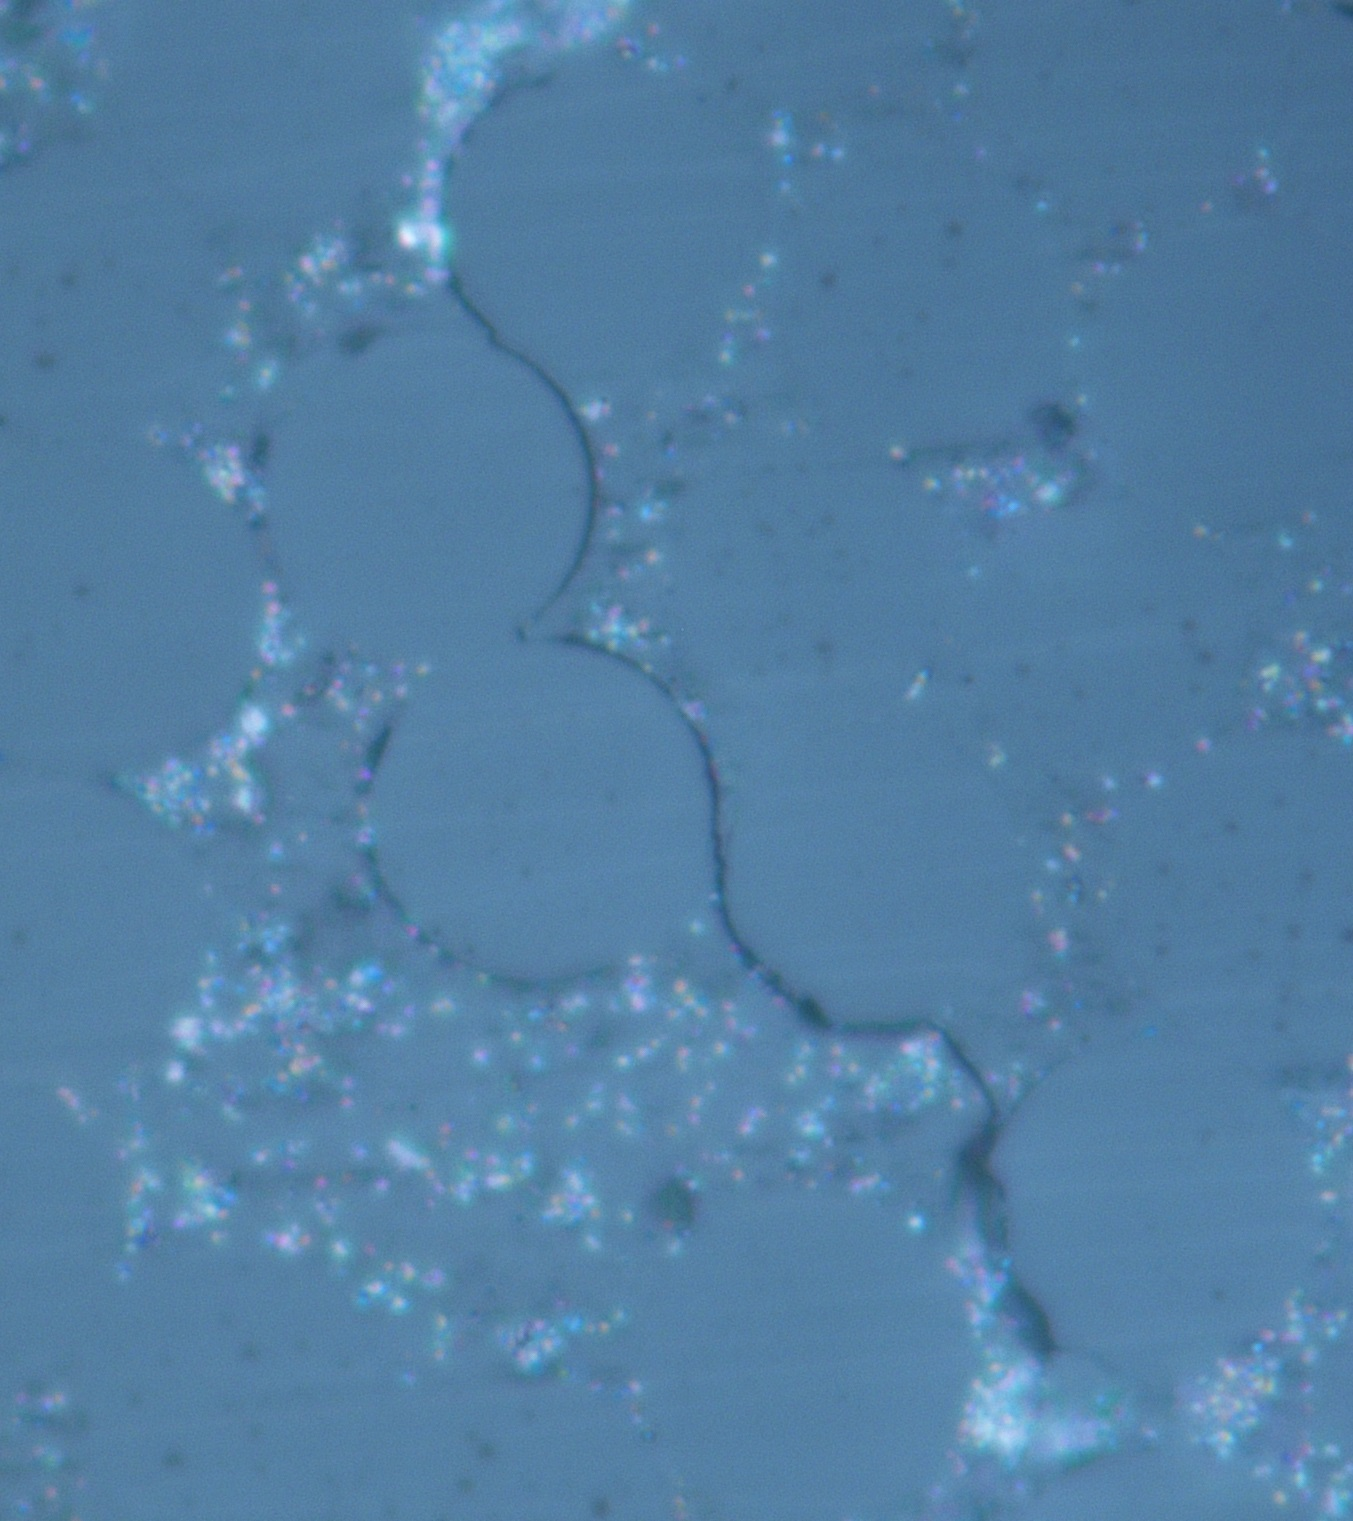
\includegraphics[height=0.6\textheight]{0-90_symm_debondetail}};
%\draw[<->,red, line width = 1.25pt] (0.075,-0.15) -- (1.1,-0.15);
%\node[red, below]  at (0.55,-0.16) {\tiny$\mathbf{\sim 8\ \mu m}$};
%\node[above, right]  at (1.2,3) {\Huge$\mathbf{\varepsilon}$};
%\node[below, left]  at (0.8,-3) {\Huge$\mathbf{\varepsilon}$};
%
%\node[anchor=south west]  at (3.25,1.55) {\scriptsize\textbf{Left:}};
%\node[anchor=west]  at (3.25,1.5) {\scriptsize front view of $\left[0,90_{2}\right]_{S}$,};
%\node[anchor=north west]  at (3.25,1.5) {\scriptsize visual inspection.};
%
%\node[anchor=south west]  at (3.25,0.05) {\scriptsize\textbf{Center:}};
%\node[anchor=west]  at (3.25,0) {\scriptsize  edge view of $\left[0,90\right]_{S}$,};
%\node[anchor=north west]  at (3.25,0) {\scriptsize optical microscope.};
%
%\node[anchor=south west]  at (3.25,-1.45) {\scriptsize\textbf{Right:}};
%\node[anchor=west]  at (3.25,-1.5) {\scriptsize edge view of $\left[0,90\right]_{S}$,};
%\node[anchor=north west]  at (3.25,-1.5) {\scriptsize optical microscope.};

%Tikz axis ends%

\end{tikzpicture}

\end{document}